\documentclass[thesis.tex]{subfiles}

\chapter{Results \& Evaluation}
\section{Experiment Setup}
To benchmark BK.Synpase's performance, we trained the presented RetinaNet architecture using the framework. The RetinaNet implementation is written in PyTorch, based on an open source implementation and slightly modified to run on both CPU and GPU for testing purposes. The modified code is available at:\\
\href{https://github.com/lanPN85/pytorch-retinanet-1}{https://github.com/lanPN85/pytorch-retinanet-1}

Due to resource constraints, we were only able to test the system on a small 2-machine setup. Both machine runs on Ubuntu Linux 18.04, which we denote as N1 and N2. They are connected via an Ethernet connection over a 100Mbps network switch. The shared data folder is on an HDD drive physically connected to N1, and mounted on N2 using Linux NFS mount. Each machine runs a BK.Synapse node daemon, while N2 also hosts the API server and the web application (Figure \ref{fig:deployment}).

\begin{table}[]
    \centering
    \begin{tabu} to \textwidth {|c|X[c]|X[c]|}
        \hline
        \textbf{Component} & \textbf{N1} & \textbf{N2} \\ \hline
        CPU & Intel Core i7-8700K, 3.70GHz & Intel Core i7-6700K, 4.00GHz \\ \hline
        CPU Cores & 6 & 4 \\ \hline
        RAM & 64GB & 32GB \\ \hline
        GPU & NVIDIA GeForce GTX 1080Ti & NVIDIA GeForce GTX 1080 \\ \hline
        GPU Memory & 12GB & 8GB \\ \hline
    \end{tabu}
    \caption{Hardware specifications for nodes N1 and N2}
    \label{tab:n1n2_specs}
\end{table}

\begin{figure}[htp]
	\centering
	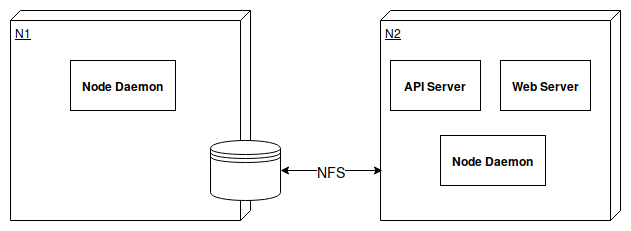
\includegraphics[width=0.9\textwidth]{deployment.png}
	\caption{Deployment diagram for our experiments}
	\label{fig:deployment}
\end{figure}
% \FloatBarrier

The training and test datasets are from ICDAR 2019 RobustReading Challenge on Scanned Receipts OCR and Information Extraction, Task 1\footnote{http://rrc.cvc.uab.es/?ch=13}. The original dataset consists of 626 images of scanned receipts, with annotations for invidual text block positions and their content. We split this data into 532 images for the train set and 94 images for the validation set. While the original challenge is to both locate each block and predict their content, we focus solely on the task of locating blocks using RetinaNet.

\begin{figure}[htp]
	\centering
	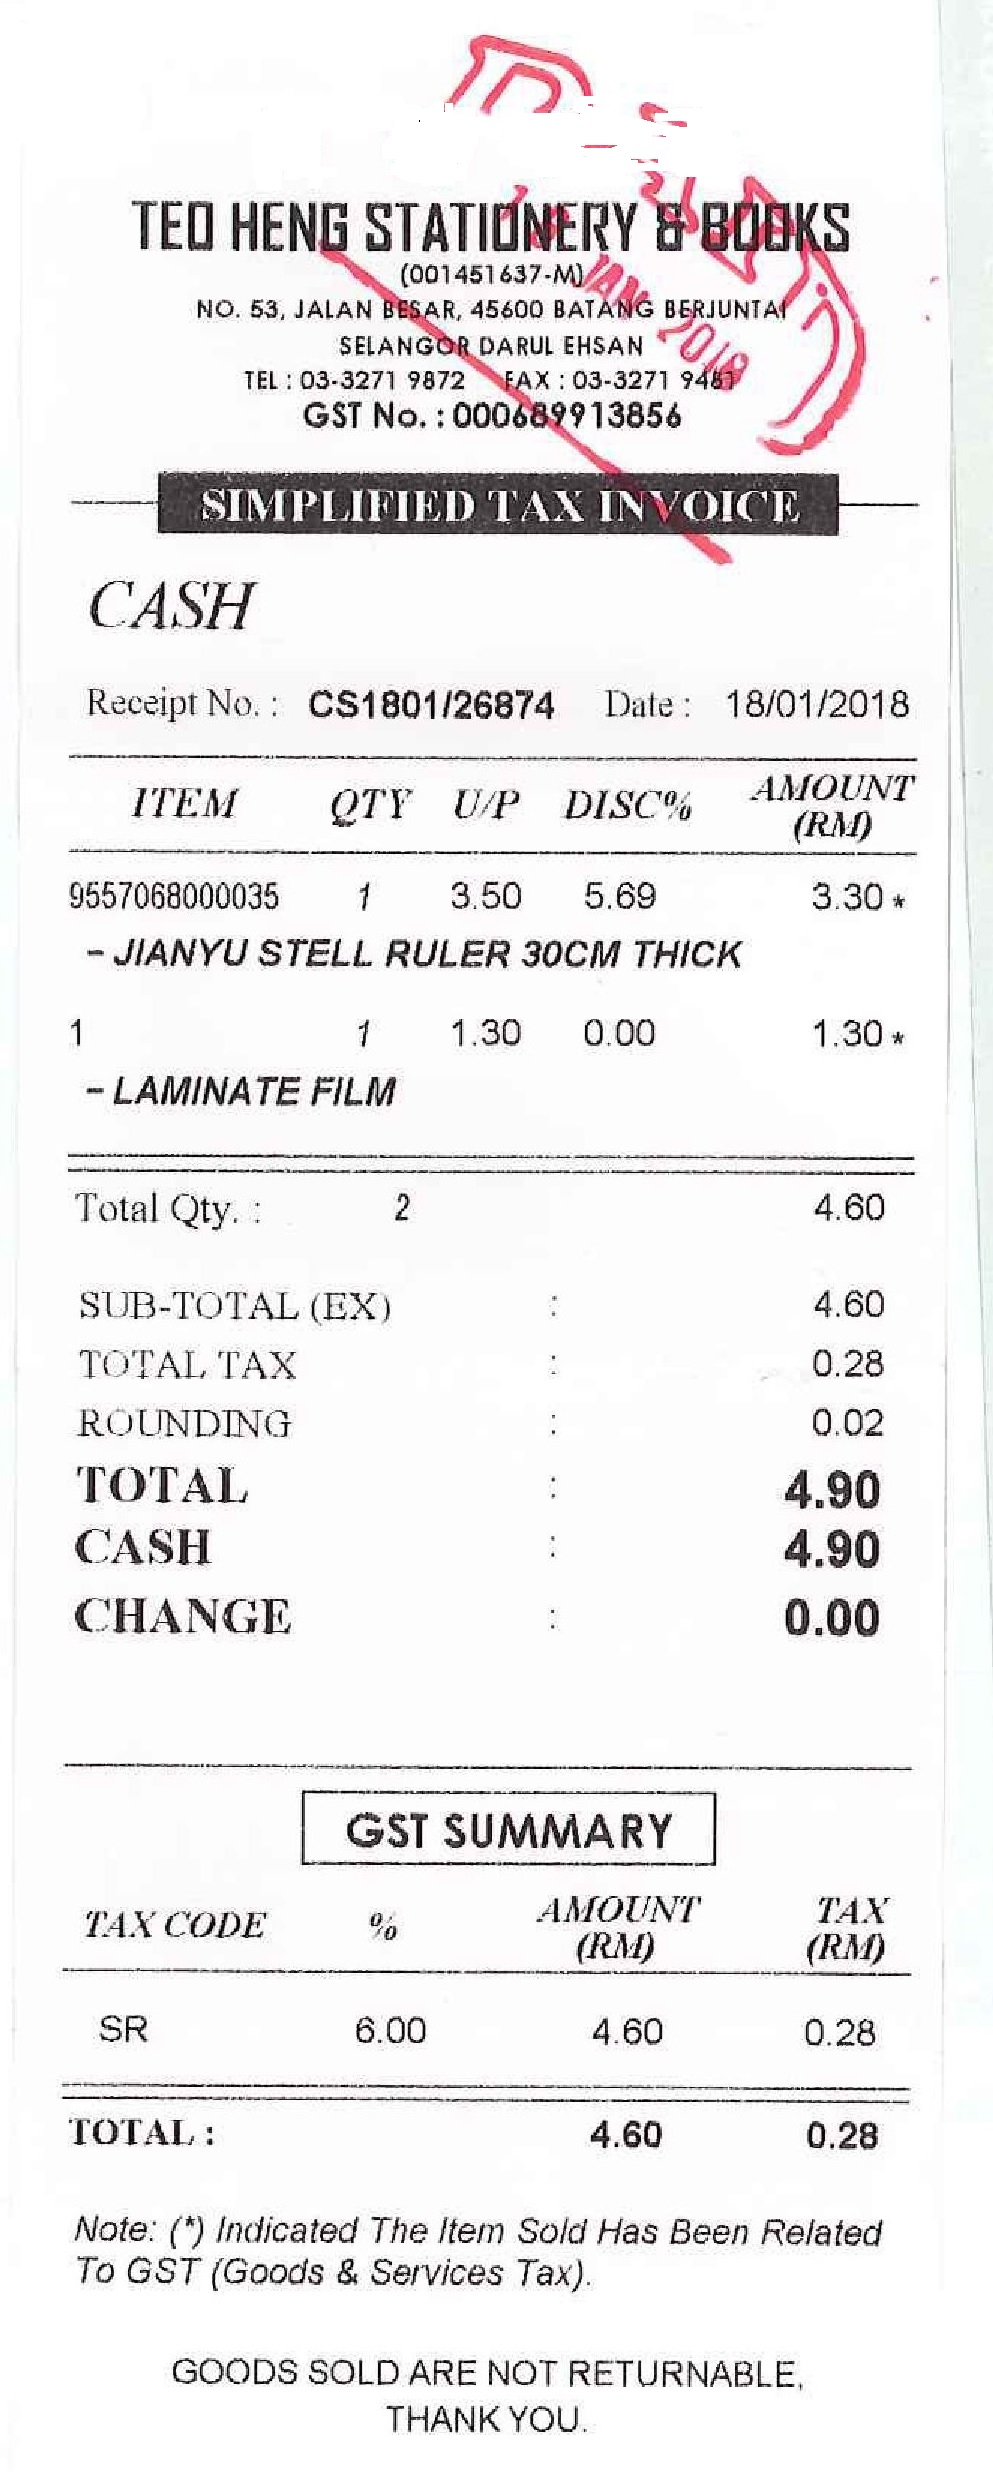
\includegraphics[width=0.2\textwidth]{data_example.jpg}
	\caption{An example scanned receipt from the ICDAR Challenge dataset}
	\label{fig:data_example}
\end{figure}

\section{Network Training Performance}
Our first set of experiments seek to benchmark BK.Synapse's performance when training a large, production-level architecture. We trained the network with 4 different resource configurations: 1 CPU, 2 CPUs, 1 GPU, and 2 GPUs. The training configurations for each run are identical as shown in Table \ref{tab:train_params}.

\begin{table}[]
\centering
\begin{tabu} to 0.8\textwidth {|X[c]|X[c]|}
    \hline
    \textbf{Parameter} & \textbf{Value} \\ \hline
    Network backbone & ResNet-50 \\ \hline
    Learning rate & 0.001 \\ \hline
    Batch size & 2 \\ \hline
    Gradient norm & 0.1 \\ \hline
    No. epochs & 10 \\ \hline
    Snapshot frequency & 2 \\ \hline
\end{tabu}
\caption{Benchmark training configuration}
\label{tab:train_params}
\end{table}
\FloatBarrier

The listed batch size is the per-node batch size. This value is quite smaller than normal, due to the size of the network and the input images. We find that a batch size of 2 avoids out-of-memory errors for our GPUs.

This benchmark is primarily concerned with parallelization metrics, including speedup and efficiency when training with multiple CPUs/GPUs, as shown in Table \ref{tab:benchmarks}. We measure the average time in seconds for each epoch and step for comparison. Speedup and efficiency are measured using per epoch time.

\begin{table}[]
    \centering
    \begin{tabu} to \textwidth {|X[c]|c|c|c|c|}
        \hline
        \textbf{Resources} & \textbf{Avg. epoch time} & \textbf{Avg. step time} & \textbf{Speedup} & \textbf{Efficiency} \\ \hline
        1 CPU & 2130.33s & 7.92s & - & - \\ \hline
        2 CPUs & - & - &  & \\ \hline
        1 GPU & 832.79 & 3.04 & - & - \\ \hline
        2 GPUs & 606.14 & 4.48 & 1.37x & 68.70\% \\ \hline
    \end{tabu}
    \caption{Benchmark time, speedup ratio and efficiency index for training RetinaNet in parallel}
    \label{tab:benchmarks}
\end{table}
\FloatBarrier

\section{Model Performance}
In our final experiment, we train the same network to convergence using BK.Synapse, and evaluate the final model's performance on the ICDAR Challenge task. We maintain the same parameters as in Table \ref{tab:train_params}, but set the number of epochs to 80. The network is trained on both N1 and N2 with GPU acceleration.
